\documentclass[conference,a4paper]{IEEEtran}
\IEEEoverridecommandlockouts

\usepackage{cite}
\usepackage{amsmath,amssymb,amsfonts}
\usepackage{algorithm}
\usepackage[noend]{algpseudocode}
\usepackage{graphicx}
\usepackage{textcomp}
\usepackage{xcolor}
\usepackage{booktabs}
\usepackage{listings}
\usepackage{tikz}
\usetikzlibrary{arrows.meta,positioning}
\usepackage{url}
\usepackage{array}
\usepackage{balance}
\newcolumntype{L}[1]{>{\raggedright\arraybackslash}p{#1}}

\newtheorem{theorem}{Theorem}
\newtheorem{lemma}{Lemma}
\newtheorem{proposition}{Proposition}

\newcommand{\QR}{\textup{\textsc{QReclaim}}}
\newcommand{\Dep}{\mathit{Dep}}
\newcommand{\Tr}{\mathit{Tr}}
\newcommand{\Lst}{L^{*}}
\newcommand{\instr}[1]{\texttt{#1}}
\makeatletter
\newcommand{\inputtable}[1]{\@@input #1 }
\makeatother
\newcommand{\NInst}{29}
\newcommand{\RedQRvsNR}{53.8}
\newcommand{\RedDNvsNR}{37.7}
\newcommand{\RedQRvsSCOPE}{42.8}
\newcommand{\RedQRvsSB}{8.3}
\newcommand{\GeoQR}{0.323}
\newcommand{\DepthQR}{2.55}
\newcommand{\DNMaxDepth}{1.0}
\newcommand{\TimeTenMin}{0.819}
\newcommand{\TimeTenMax}{2.194}
\newcommand{\MaxCompileMs}{42.4}
\newcommand{\MaxDNSearchMs}{4375.6}
\newcommand{\MainSim}{59}
\newcommand{\MainTotal}{145}
\newcommand{\VerSim}{35}
\newcommand{\VerTotal}{36}
\newcommand{\MaxTVD}{1.3\times10^{-14}}
\newcommand{\VerMaxAer}{0.027}
\newcommand{\FreesValidated}{1944}
\newcommand{\Slope}{1.03}
\newcommand{\UsPerInstr}{10.3}
\newcommand{\KneeBV}{33}
\newcommand{\KneeHS}{75}
\newcommand{\KneeRC}{59}
\newcommand{\KneeGRV}{51}
\newcommand{\MutN}{237}
\newcommand{\MutFaulty}{175}
\newcommand{\MutFP}{10}
\newcommand{\MutRecall}{100.0}
\newcommand{\MutPrecision}{94.6}


\lstdefinestyle{base}{basicstyle=\ttfamily\scriptsize, columns=fullflexible, keepspaces=true,
  commentstyle=\color{black!55}\itshape, xleftmargin=0pt, aboveskip=1pt, belowskip=1pt,
  showstringspaces=false}
\lstdefinestyle{ir}{style=base, morecomment=[l]{;}}
\lstdefinestyle{dsl}{style=base, language=Python, keywordstyle=\bfseries}

\begin{document}

\title{Memory Management and Garbage Collection Strategies in High-Level Quantum Programming Languages}

\author{\IEEEauthorblockN{Rajveer Chopra}
\IEEEauthorblockA{Reg. No.: 24BCE0122\\
\textit{School of Computer Science and Engineering (SCOPE)}\\
\textit{Vellore Institute of Technology}\\
Vellore, Tamil Nadu, India\\
rajveer.singhchopra2024@vitstudent.ac.in}}

\maketitle

\begin{abstract}
High-level quantum languages let programmers allocate temporary qubits as freely as local variables. Returning those qubits is a memory-management problem without a classical counterpart: a live qubit cannot be copied, inspected or silently dropped, so neither copying nor tracing garbage collection applies. This paper presents \QR{}, a compile-time garbage collector for qubits built on a linear intermediate representation (QR-IR). A forward basis-state abstract interpretation computes, for every ancilla, the reversible trace that produced it, its dependencies and an uncomputation deadline. An uncomputation-aware extension of live-variable analysis then places each uncomputation at the earliest provably safe point. The same framework reclaims measured qubits by early measurement and reset, deletes ancillas that are never read, and statically validates that every freed qubit is $|0\rangle$. An earliest-ready-first linear-scan allocator exposes the width--depth trade-off as a single qubit budget. On six benchmark families (\NInst{} instances) \QR{} reduces the number of physical qubits by \RedQRvsNR\% on average relative to compilation without reuse, and its depth-neutral mode saves \RedDNvsNR\% with no increase in depth. A bug-injection study shows that the static checks detect all \MutFaulty{} faulty mutants at \MutPrecision\% precision.
\end{abstract}

\begin{IEEEkeywords}
quantum compilers, uncomputation, qubit reuse, garbage collection, data-flow analysis, register allocation, no-cloning theorem
\end{IEEEkeywords}

%% =====================================================================
\section{Introduction}
\label{sec:intro}
Quantum processors offer tens to a few hundred qubits, so the number of qubits a program needs (its \emph{width}) decides whether it can run at all. At the same time, programs are increasingly written in high-level languages such as Silq~\cite{silq}, Qrisp~\cite{qrisp} and Qurts~\cite{qurts}, where temporary qubits (\emph{ancillas}) are declared like local variables and returned automatically. Returning them safely and early is the quantum analogue of memory management.

Classical garbage collection does not carry over. A copying collector moves objects, but a quantum state cannot be copied~\cite{wootters1982}. A tracing collector inspects the heap, but measuring a qubit disturbs it. Above all, a dead temporary is usually \emph{entangled} with live data, and discarding it destroys the interference that quantum algorithms rely on. Such a qubit can be freed only by \emph{uncomputing} it, i.e.\ running the gates that produced it in reverse~\cite{bennett1973}, which is valid only while its inputs are unchanged. Mid-circuit measurement and reset offer a second route for qubits whose value is no longer needed coherently~\cite{caqr,decross2023}. A compiler must therefore answer four questions:
\begin{enumerate}
\item \emph{Safety:} when can a qubit be reclaimed without aliasing two states onto one qubit or leaving entangled garbage behind?
\item \emph{Placement:} where between an ancilla's last use and the next write to its inputs should its uncomputation go, given that ancillas computed from other ancillas extend each other's lifetimes?
\item \emph{Unification:} can uncomputation-based and measurement-based reclamation be decided by one analysis?
\item \emph{Allocation:} reusing a qubit serialises work that could run in parallel (a false dependency, as in register allocation). How should width be traded against depth?
\end{enumerate}

\QR{} answers these with standard compiler machinery adapted to quantum constraints. Its contributions are:
\begin{itemize}
\item a \textbf{linear IR with static semantics} whose typing rules forbid aliasing and whose \textsc{T-Free} rule is discharged by a static validator, so a freed qubit is provably $|0\rangle$ (\S\ref{sec:ir}--\ref{sec:types});
\item a \textbf{basis-state abstract interpretation and an uncomputation-aware liveness analysis}, written as data-flow equations with a legality condition and a soundness argument (\S\ref{sec:analysis});
\item a \textbf{unified reclamation pass} for uncomputation, early measurement and reset, and dead-garbage elimination, applied hierarchically before and after the lowering of multi-controlled gates (\S\ref{sec:reclaim});
\item an \textbf{earliest-ready-first (ERF) linear-scan allocator} with an explicit qubit budget and a depth-neutral mode (\S\ref{sec:alloc});
\item an \textbf{evaluation} against no reuse, lexical reclamation, a strong baseline that combines prior techniques, and the external framework Qrisp, plus a bug-injection study of the static checks (\S\ref{sec:results}).
\end{itemize}

%% =====================================================================
\section{Literature Review}
\label{sec:lit}

\subsection{High-level languages and uncomputation}
Silq~\cite{silq} introduced safe automatic uncomputation. Its \texttt{qfree} and \texttt{const} annotations identify reversible computations and unchanged inputs, temporaries are uncomputed implicitly, and unphysical programs are rejected by the type system. Qurts~\cite{qurts} carries Rust-style affine types with lifetimes over to qubits: inside its lifetime a value may be dropped and is then uncomputed automatically. Qrisp~\cite{qrisp} is a Python-embedded framework whose uncomputation follows the Unqomp approach~\cite{unqomp}. Its compiler maps qubits of deleted variables onto free physical qubits, and its \texttt{workspace} option grants extra qubits to reduce depth. Unqomp~\cite{unqomp} synthesises uncomputation on a circuit graph, Reqomp~\cite{reqomp} adds a space constraint and trades recomputation for ancillas, and SQUARE~\cite{square} decides at each call site whether to uncompute or keep garbage using a cost model that accounts for locality and parallelism. All of these build on Bennett's compute--copy--uncompute construction~\cite{bennett1973}.

\subsection{Qubit reuse by measurement and reordering}
CaQR~\cite{caqr} reuses a qubit after its final measurement by inserting a reset, and reports resource reductions of up to 80\%. DeCross \emph{et al.}~\cite{decross2023} formulate measurement-based reuse exactly as a constraint program and greedily. Jiang~\cite{jiang2024} recasts circuit-level qubit recycling as matrix triangularisation, proves it NP-hard and gives a dependency-graph heuristic, which justifies heuristic reordering. Closest to our scheduler, Reichental \emph{et al.}~\cite{classiq2025} search for a topological order of a high-level program that maximises the reuse of uncomputed qubits, with heuristics that trade width for depth.

\subsection{Compiler frameworks and static analysis techniques}
Industrial frameworks such as Qiskit~\cite{qiskit2024} compile through a pass manager over a DAG IR. They lower and optimise circuits but treat qubits as fixed registers, so they do not reclaim them. Static analysis of quantum programs is mostly \emph{semantic}: Yu and Palsberg~\cite{yupalsberg2021} define an abstract interpretation whose abstract states are projections on small qubit subsets, which lets assertions be verified in polynomial time. Our analysis is \emph{structural} instead. It tracks reversible traces, dependencies and lifetimes, which is what reclamation needs, and it transfers classical live-variable analysis and linear-scan register allocation~\cite{linearscan} to qubits. Two classical notions do not carry over: spilling is impossible because states cannot be copied, and freeing requires uncomputation or measurement.

\subsection{Identified research gaps}
Table~\ref{tab:lit} summarises the mechanisms. Three gaps motivate this work:
\begin{enumerate}
\item[\textbf{G1}] Uncomputation-based reuse~\cite{unqomp,reqomp,square,qrisp} and measurement-based reuse~\cite{caqr,decross2023,jiang2024} are developed as separate passes at different abstraction levels.
\item[\textbf{G2}] Reclamation legality is stated as type rules~\cite{silq,qurts} or circuit-graph conditions~\cite{unqomp} rather than as data-flow facts that compose with the liveness, scheduling and allocation passes of a conventional compiler.
\item[\textbf{G3}] Static guarantees that a freed qubit is clean, and diagnostics for programs where no safe reclamation exists, are tied to specific languages, and their precision is rarely measured.
\end{enumerate}

\begin{table}[t]
\caption{Qubit-reclamation mechanisms in related work}
\label{tab:lit}
\centering
\scriptsize
\setlength{\tabcolsep}{3pt}
\begin{tabular}{@{}L{1.9cm}L{2.6cm}L{3.6cm}@{}}
\toprule
Work & Mechanism & Decision basis \\
\midrule
Silq~\cite{silq}, Qurts~\cite{qurts} & implicit uncomputation & type system; lexical scope / lifetime \\
Qrisp~\cite{qrisp} & uncomputation, recycling & Unqomp-style synthesis; workspace knob \\
Unqomp~\cite{unqomp}, Reqomp~\cite{reqomp} & uncomputation (+ recompute) & circuit graph; ancilla budget \\
SQUARE~\cite{square} & uncompute or keep & cost model at call sites \\
CaQR~\cite{caqr}, DeCross~\cite{decross2023} & measure + reset & circuit DAG; exact / greedy \\
Jiang~\cite{jiang2024}, Classiq~\cite{classiq2025} & reordering for reuse & dependency graph; topological sort \\
\midrule
\textbf{\QR{}} & uncompute, measure + reset, DGE & data-flow window (Eq.~\ref{eq:legal}), static validation, ERF budget \\
\bottomrule
\end{tabular}
\end{table}

%% =====================================================================
\section{Proposed Model / Architecture}
\label{sec:model}

\subsection{System overview}
Fig.~\ref{fig:arch} shows the pipeline. Programs written in an embedded front end become QR-IR, a straight-line list of instructions over \emph{logical} qubits. A linear type check rejects aliasing. A forward basis-state analysis and a backward liveness analysis then drive the \emph{level-1 reclamation pass}, which inserts uncomputations, early measurements, resets and \instr{free}s for programmer ancillas, and a static validator proves every inserted \instr{free} safe. Multi-controlled gates are then lowered to Toffoli chains, and the same pass and validator reclaim the helper qubits this creates (level~2). Finally, a pressure-aware scheduler reorders commuting instructions, an ERF linear-scan allocator maps logical to physical qubits under an optional budget, and code is emitted as a Qiskit circuit or OpenQASM~2.

\begin{figure*}[t]
\centering
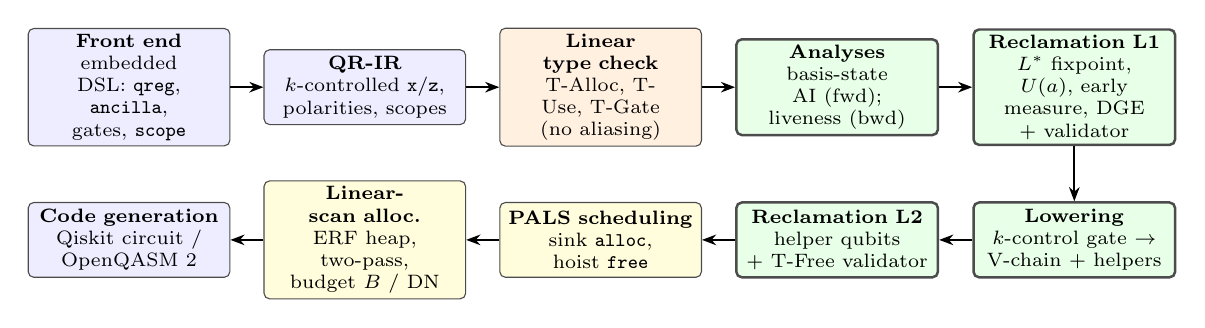
\begin{tikzpicture}[
  node distance=3mm and 4.2mm,
  st/.style={draw=black!70, rounded corners=2pt, align=center, font=\scriptsize,
             minimum height=9.5mm, text width=24.2mm, inner sep=2pt},
  fe/.style={st, fill=blue!7}, gc/.style={st, fill=green!9, line width=0.9pt},
  tc/.style={st, fill=orange!12}, be/.style={st, fill=yellow!14},
  arr/.style={-{Stealth[length=1.8mm]}, semithick}]
\node[fe] (fe) {\textbf{Front end}\\ embedded DSL: \texttt{qreg},\\ \texttt{ancilla}, gates, \texttt{scope}};
\node[fe, right=of fe] (ir) {\textbf{QR-IR}\\ $k$-controlled \texttt{x}/\texttt{z},\\ polarities, scopes};
\node[tc, right=of ir] (tc) {\textbf{Linear type check}\\ T-Alloc, T-Use, T-Gate\\ (no aliasing)};
\node[gc, right=of tc] (an) {\textbf{Analyses}\\ basis-state AI (fwd);\\ liveness (bwd)};
\node[gc, right=of an] (r1) {\textbf{Reclamation L1}\\ $\Lst$ fixpoint, $U(a)$, early\\ measure, DGE + validator};
\node[gc, below=7mm of r1] (lo) {\textbf{Lowering}\\ $k$-control gate $\to$\\ V-chain + helpers};
\node[gc, left=of lo] (r2) {\textbf{Reclamation L2}\\ helper qubits\\ + T-Free validator};
\node[be, left=of r2] (sc) {\textbf{PALS scheduling}\\ sink \texttt{alloc},\\ hoist \texttt{free}};
\node[be, left=of sc] (al) {\textbf{Linear-scan alloc.}\\ ERF heap, two-pass,\\ budget $B$ / DN};
\node[fe, left=of al] (cg) {\textbf{Code generation}\\ Qiskit circuit /\\ OpenQASM 2};
\foreach \a/\b in {fe/ir, ir/tc, tc/an, an/r1, r1/lo, lo/r2, r2/sc, sc/al, al/cg} \draw[arr] (\a) -- (\b);
\end{tikzpicture}
\caption{The \QR{} pipeline. Stages with a bold border form the compile-time garbage collector; the same reclamation pass and validator run at two IR levels. A physical no-aliasing check and dead-reset elimination follow allocation.}
\label{fig:arch}
\end{figure*}

\subsection{Intermediate representation (QR-IR)}
\label{sec:ir}
A QR-IR program is a sequence $P=\iota_0\ldots\iota_{N-1}$ of
\begin{align*}
\iota ::=\;& \instr{alloc}\ q \mid \instr{free}\ q \mid g^{\theta}(\bar c^{\,\bar\pi};\bar t)\\
 \mid\;& \instr{measure}\ q\to c \mid \instr{reset}\ q
\end{align*}
where $\bar c$ are controls with polarities $\pi\in\{+,-\}$ (a $-$ control fires on $|0\rangle$), $\bar t$ are targets and $\theta$ optional angles. CX, Toffoli and $k$-controlled X are the same base operation $\instr{x}$ with $|\bar c|=1,2,k$. Qubits are \emph{data} (owned by the programmer), \emph{ancillas} (reclaimed by the compiler) or \emph{helpers} (created by lowering). Gates fall into three classes by their action on computational-basis states: $G_{\mathrm{qf}}=\{\instr{x},\instr{swap}\}$ \emph{permute} the basis; $G_{\mathrm{dg}}=\{\instr{z},\instr{s},\instr{t},\instr{rz},\instr{p}\}$ and their inverses are \emph{diagonal}; $G_{\mathrm{gen}}=\{\instr{h},\instr{rx},\instr{ry}\}$ may create superposition. The \emph{write set} $W(\iota)$ contains the targets of $G_{\mathrm{qf}}\cup G_{\mathrm{gen}}$ gates and of \instr{reset}; controls and diagonal gates never write. Negative controls stay symbolic until code generation, so their $X$ conjugation is never mistaken for a write. QR-IR has no classically controlled operations, so after inlining and unrolling a program is a single basic block. Programmers write only the forward computation and never uncompute or free (Fig.~\ref{fig:example}).

\subsection{Static semantics}
\label{sec:types}
Judgements $\Delta\vdash\iota\dashv\Delta'$ thread a context mapping each live qubit to its abstract state (\S\ref{sec:ai}):
\begin{gather*}
\frac{q\notin\mathrm{dom}(\Delta)}{\Delta\vdash \instr{alloc}\ q\dashv \Delta,q{:}\mathbf{0}}\,\textsc{(T-Alloc)}
\\[3pt]
\frac{q\in\mathrm{dom}(\Delta)}{\Delta\vdash \instr{measure}\ q \dashv \Delta[q\mapsto\mathbf{M}]}\,\textsc{(T-Use)}\\[3pt]
\frac{\bar c,\bar t\ \text{pairwise distinct}\quad \{\bar c,\bar t\}\subseteq\mathrm{dom}(\Delta)}{\Delta\vdash g(\bar c;\bar t)\dashv \Delta[\bar t\mapsto \tau_g(\Delta,\bar t)]}\,\textsc{(T-Gate)}
\\[3pt]
\frac{\vdash_{\!\mathit{XOR}} q\ \text{clean}}{\Delta\vdash \instr{free}\ q\dashv \Delta\setminus q}\,\textsc{(T-Free)}
\end{gather*}
\textsc{T-Use} also covers \instr{reset}, which sets the state to $\mathbf{0}$. The state transformer $\tau_g$ is that of Table~\ref{tab:transfer}: $G_{\mathrm{qf}}$ yields $\mathbf{B}$ (or $\mathbf{T}$), $G_{\mathrm{gen}}$ yields $\mathbf{T}$, and $G_{\mathrm{dg}}$ changes nothing. Since QR-IR has no copy instruction, no program can clone a state~\cite{wootters1982}. The rules guarantee the two properties a qubit manager needs instead: an operation never uses one qubit in two roles, and a qubit is freed, and later handed out again, only when it is provably $|0\rangle$. The premise of \textsc{T-Free} is discharged by the validator of \S\ref{sec:validate}. After allocation, a physical variant of the check verifies that no physical qubit hosts two live logical qubits.

\subsection{Data-flow analyses}
\label{sec:analysis}

\subsubsection{Basis-state abstract interpretation (forward)}
\label{sec:ai}
Each qubit carries a state $\sigma(q)$ in the lattice $\bot\sqsubseteq\mathbf{0}\sqsubseteq\mathbf{B}\sqsubseteq\mathbf{T}$, $\bot\sqsubseteq\mathbf{M}\sqsubseteq\mathbf{T}$, where $\bot$ means unallocated, $\mathbf{0}$ exactly $|0\rangle$, $\mathbf{B}$ a basis value that is a reversible function of other qubits, $\mathbf{M}$ measured and $\mathbf{T}$ possibly in superposition. It also carries a \emph{trace} $\Tr(q)$ (the qfree gates that computed it), a \emph{dependency set} $\Dep(q)$ (their controls) and a \emph{deadline} $D(q)$: the first later position that writes some $d\in\Dep(q)$. With $\mathrm{IN}[0]=\bot^{Q}$, $\mathrm{OUT}[i]=f_{\iota_i}(\mathrm{IN}[i])$ and $\mathrm{IN}[i{+}1]=\mathrm{OUT}[i]$, one forward sweep computes all facts; Table~\ref{tab:transfer} gives $f_\iota$. Clearing the reverse map from a written qubit to its dependants keeps the deadline bookkeeping amortised $O(1)$ per instruction.

\begin{table}[t]
\caption{Transfer functions $f_\iota$ of the basis-state analysis ($\iota$ at position $i$)}
\label{tab:transfer}
\centering
\scriptsize
\setlength{\tabcolsep}{3pt}
\begin{tabular}{@{}L{2.9cm}L{5.4cm}@{}}
\toprule
Instruction $\iota$ & Effect \\
\midrule
\instr{alloc} $q$ & $\sigma(q){\gets}\mathbf{0}$;\ $\Tr(q){\gets}\epsilon$;\ $\Dep(q){\gets}\emptyset$;\ $D(q){\gets}\infty$ \\
$g(\bar c;t)$, $g\in G_{\mathrm{qf}}$, $\sigma(t)\in\{\mathbf{0},\mathbf{B}\}$, $D(t)=\infty$ & $\sigma(t){\gets}\mathbf{B}$;\ $\Tr(t){\gets}\Tr(t)\cdot\iota$;\ $\Dep(t){\gets}\Dep(t)\cup\bar c$ \\
other qfree gate; $g\in G_{\mathrm{gen}}$ & $\sigma(t){\gets}\mathbf{T}$ for every target $t$ \\
$g\in G_{\mathrm{dg}}$ & no change (adds phases only) \\
\instr{measure} $q$ & $\sigma(q){\gets}\mathbf{M}$ \\
\instr{reset} $q$ & $\sigma(q){\gets}\mathbf{0}$;\ $\Tr(q){\gets}\epsilon$;\ $\Dep(q){\gets}\emptyset$;\ $D(q){\gets}\infty$ \\
any $\iota$, each $w\in W(\iota)$ & for all $a$ with $w\in\Dep(a)$, $D(a)=\infty$: $D(a){\gets}i$ \\
\bottomrule
\end{tabular}
\end{table}

\subsubsection{Liveness (backward)}
With $\mathit{DEF}(\iota)=\{q\}$ for $\instr{alloc}\ q$ and $\mathit{USE}(\iota)$ the operands of every other instruction:
\begin{align}
\mathit{LIVE}_{in}(\iota) &= \mathit{USE}(\iota)\cup\big(\mathit{LIVE}_{out}(\iota)\setminus \mathit{DEF}(\iota)\big),\label{eq:live1}\\
\mathit{LIVE}_{out}(\iota_i) &= \mathit{LIVE}_{in}(\iota_{i+1}),\label{eq:live2}\\
L(q) &= \max\{\,i : q\in \mathit{USE}(\iota_i)\,\}.\label{eq:lastuse}
\end{align}
One backward sweep yields every last use $L(q)$.

\subsubsection{Uncomputation-aware liveness and placement}
Inserting the uncomputation $U(a)$ of ancilla $a$ at position $P(a)$ \emph{reads} every $d\in\Dep(a)$ again, so the last use of a dependency can move later. For the set $R$ of ancillas to uncompute, the effective last use is the least fixpoint of
\begin{align}
\Lst(q) &= \max\big(L(q),\ \max\{P(a): a\in R,\ q\in\Dep(a)\}\big),\label{eq:lstar}\\
P_{\mathrm{eager}}(a) &= \Lst(a),\label{eq:eager}\\
P_{\mathrm{lazy}}(a) &= \min\big(\mathit{end}(\mathit{scope}(a)),\ D(a){-}1,\nonumber\\
 &\qquad\ \min\{P_{\mathrm{lazy}}(b): b\in\Dep(a)\cap R\}\big),\label{eq:lazy}
\end{align}
and a placement is \emph{legal} iff
\begin{equation}
\Lst(a)\ \le\ P(a)\ <\ D(a)\qquad\text{for every } a\in R. \label{eq:legal}
\end{equation}
Eq.~(\ref{eq:eager}) is \QR{}'s policy; Eq.~(\ref{eq:lazy}) models lexical reclamation. If (\ref{eq:legal}) fails, the program is rejected with a diagnostic naming the instruction that overwrote the input. The fixpoint is solved round-robin: $P$ only grows and is bounded by $N$, so it terminates within $h{+}1$ sweeps for a dependency DAG of height $h$. On all our benchmarks one productive sweep plus one confirming sweep sufficed.

\begin{theorem}[Sound uncomputation]\label{thm:sound}
Let every $a\in R$ satisfy (\ref{eq:legal}), with $\sigma(a)=\mathbf{B}$ and $U(a)=\Tr(a)_k^{-1}\cdots\Tr(a)_1^{-1}$, and let blocks inserted at the same point be ordered so that a block reading $q$ precedes the block writing (freeing) $q$. Then at each $\instr{free}\ a$ the ancilla is $|0\rangle$ and unentangled. Moreover the final state of the other qubits does not depend on which legal $P(a)$ is chosen.
\end{theorem}
\begin{IEEEproof}[Proof sketch]
Every $b$ with $a\in\Dep(b)$ satisfies $P(b)\le\Lst(a)\le P(a)$, and a reset of some $d\in\Dep(a)$ is placed after $P(a)$, so no instruction, original or inserted, writes $\Dep(a)$ between the first trace gate and $U(a)$. Expand the state in the computational basis of $\Dep(a)$. In each branch $|d\rangle$, every trace gate sees the same control values when applied and when reversed. Every other operation on $a$ only reads it (as a control or through a diagonal gate), since a write would have made $\sigma(a)=\mathbf{T}$. So $U(a)$ maps $|d\rangle|f(d)\rangle\mapsto|d\rangle|0\rangle$, and by linearity the state factorises as $|\psi\rangle\otimes|0\rangle_a$. Within the window, other instructions touch $\Dep(a)$ only as controls, through diagonal gates or by measurement. They and $U(a)$ are block-diagonal in that basis and act on disjoint qubits within each block, so they commute.
\end{IEEEproof}

\begin{lemma}[Early measurement]\label{lem:meas}
If the final operation on $q$ is $\instr{measure}$ at $m$ and its previous use is at $\ell<m$, moving the measurement to just after $\max(\ell,\max\{P(b):q\in\Dep(b)\})$ and appending $\instr{reset}\ q;\ \instr{free}\ q$ preserves the joint outcome distribution and the state of all other qubits, because measurement commutes with operations on disjoint qubits and with operations that use $q$ only as a control.
\end{lemma}

\subsection{Reclamation transformations}
\label{sec:reclaim}
Algorithm~\ref{alg:reclaim} summarises the pass, which is parameterised by the qubit kinds it manages.

\emph{Dead-garbage elimination (DGE).} An ancilla whose only uses are its own trace gates is never read, so its computation and its uncomputation would cancel. Both are deleted together with the allocation, as for the unused carry-out of an adder.

\emph{Uncomputation, measurement and diagnostics.} For each $a\in R$ the pass inserts $U(a);\ \instr{free}\ a$ after $\iota_{P(a)}$, applies Lemma~\ref{lem:meas} to every qubit whose final operation is a measurement, and orders blocks at a shared point so that readers come before writers (every block ends in a \instr{free}, which counts as a write). An ancilla that ends in $\mathbf{T}$ and is never measured is reported statically instead of being leaked.

\emph{Hierarchical reclamation.} A gate with $k\ge3$ controls is lowered to a V-chain of $k{-}2$ helpers and one Toffoli or CCZ. Lowering emits only the compute half; running Algorithm~\ref{alg:reclaim} again on helpers produces the uncompute half. Level~1 must run \emph{before} lowering: there, a clause ancilla computed by a 3-controlled gate depends only on its inputs, whereas after lowering it would also depend on a helper, keeping that helper alive.

\begin{algorithm}[t]
\caption{\textsc{Reclaim}$(P,K,\mathit{mode})$}
\label{alg:reclaim}
\footnotesize
\begin{algorithmic}[1]
\State $(\sigma,\Tr,\Dep,D)\gets\textsc{BasisAI}(P)$;\ \ $L\gets\textsc{Liveness}(P)$
\State $G\gets\{a\in K:\sigma(a)\in\{\mathbf{0},\mathbf{B}\}\wedge \mathit{uses}(a)=\Tr(a)\}$;\ delete $\Tr(a)$, $\instr{alloc}\ a$ for $a\in G$
\If{$\exists a\in K\setminus G:\sigma(a)=\mathbf{T}$} \textbf{error} ``unreclaimable ancilla'' \EndIf
\State $R\gets\{a\in K\setminus G:\sigma(a)=\mathbf{B}\}$
\If{$\mathit{mode}=\textsc{eager}$}
  \Repeat\ \ \textbf{for} $a\in R$: $P(a)\gets\max(L(a),\max\{P(b):a\in\Dep(b)\})$
  \Until{no $P(a)$ changed}
\Else\ \ $P(a)\gets$ Eq.~(\ref{eq:lazy}) by memoised recursion
\EndIf
\State \textbf{check} Eq.~(\ref{eq:legal}) for all $a\in R$, \textbf{else error} naming $D(a)$
\ForAll{$q$ whose final operation is $\instr{measure}$ at $m$}
  \State move $\iota_m$ after $\max(\mathit{uses}(q)\setminus\{m\}\cup\{P(b):q\in\Dep(b)\})$; append $\instr{reset}\ q;\ \instr{free}\ q$
\EndFor
\State insert $U(a);\ \instr{free}\ a$ after $\iota_{P(a)}$ for all $a\in R$, readers before writers
\end{algorithmic}
\end{algorithm}

\subsection{Static validation of frees}
\label{sec:validate}
Rather than trusting the pass, \QR{} validates its output (translation validation). For each \instr{free}~$a$, consider the operations on $a$ since its last \instr{alloc} or \instr{reset}. They must be X-type writes $a\mathrel{\oplus}=\textstyle\bigwedge(\bar c^{\bar\pi})$, uses of $a$ as a control, or diagonal gates. Every control pattern $(\bar c,\bar\pi)$ must occur an even number of times, and no control of a pattern may be written between that pattern's first and last occurrence. Each term is then XORed in an even number of times with identical control values on every basis branch, so $a$ is $|0\rangle$ and unentangled, which discharges \textsc{T-Free}. The validator runs after both reclamation levels in every compilation.

\subsection{Scheduling and allocation}
\label{sec:alloc}
\emph{Pressure-aware list scheduling (PALS).} Gates on disjoint qubits commute, so any topological order of the per-qubit precedence DAG is equivalent to the input. PALS emits ready instructions in order of their effect on the number of live qubits: \instr{free} ($-1$) before other operations ($0$, in source order) before \instr{alloc} ($+1$, ordered by first use). This sinks allocations and hoists reclamation, the program-level counterpart of CaQR's reuse pairs~\cite{caqr} and of reordering for recycling~\cite{jiang2024,classiq2025}.

\emph{ERF linear scan.} After scheduling, each logical qubit occupies one interval $[\instr{alloc},\instr{free}]$, so interference forms an interval graph.

\begin{proposition}\label{prop:opt}
For a fixed order, let $\omega=\max_i|A(i)|$, where $A(i)$ is the set of qubits allocated but not freed at position $i$. Linear scan that reuses a free physical qubit whenever one exists uses exactly $\omega$ qubits, the minimum~\cite{linearscan}. A second pass with budget $B=\omega$ that takes fresh qubits first never fails.
\end{proposition}

When the allocator reuses a qubit, it takes the pooled qubit whose last operation finishes earliest in the ASAP schedule (earliest-ready-first). This minimises the false dependency the reuse creates, and a min-heap gives $O(\log n)$ selection, since a pooled qubit's ready time cannot change. With a budget $B$, fresh qubits are used until $B$ exist. \emph{\QR{}-min} uses $B=\omega$. \emph{\QR{}-DN} (depth-neutral) scans $B$ upwards for the smallest budget whose circuit is no deeper than the no-reuse circuit. A linear scan is used because depth is not monotone in $B$. Resets on qubits that are never handed out again are removed afterwards. With $N$ instructions, analyses and checks are $O(N)$ and scheduling and allocation $O(N\log N)$.

\begin{figure}[t]
\centering
\begin{lstlisting}[style=dsl]
x = p.qreg("x", 2); y = p.qreg("y", 2)
for q in x + y: p.h(q)
with p.scope():                     # oracle (-1)^{x.y}
    for i in range(2):
        t = p.ancilla("t")          # never freed by hand
        p.ccx(x[i], y[i], t); p.z(t)
for q in x + y: p.h(q); p.measure(q)
\end{lstlisting}
\vspace{1pt}
\begin{minipage}[t]{0.43\columnwidth}
\textbf{(b)} SCOPE: 6 qubits
\begin{lstlisting}[style=ir]
alloc t0           ; q4
ccx x0,y0 -> t0; z t0
alloc t1           ; q5
ccx x1,y1 -> t1; z t1
ccx x1,y1 -> t1    ; U(t1)
ccx x0,y0 -> t0    ; U(t0)
free t1; free t0
h ...; measure ...
\end{lstlisting}
\end{minipage}\hfill
\begin{minipage}[t]{0.55\columnwidth}
\textbf{(c)} \QR{}: 5 qubits
\begin{lstlisting}[style=ir]
alloc t0           ; q4
ccx x0,y0 -> t0; z t0
ccx x0,y0 -> t0    ; U(t0)
free t0            ; q4 freed
h x0; measure x0   ; hoisted
h y0; measure y0   ; hoisted
alloc t1           ; q4 reused
ccx x1,y1 -> t1; z t1; U(t1)
\end{lstlisting}
\end{minipage}
\caption{Worked example (condensed compiler output). (a) Source with two implicit temporaries. (b) Lexical reclamation keeps both until scope end. (c) \QR{} reclaims $t_0$ at its last use and reuses its qubit for $t_1$.}
\label{fig:example}
\end{figure}

%% =====================================================================
\section{Implementation / Experimental Setup}
\label{sec:impl}
\emph{Toolchain.} \QR{} is about 1{,}500 lines of Python~3.13, one module per stage of Fig.~\ref{fig:arch}. We use a custom pass pipeline rather than LLVM or GCC because reclamation needs linear qubit values, qubit kinds and uncomputation, none of which LLVM IR models. Code generation targets Qiskit~2.5.2~\cite{qiskit2024}, which also lowers every output to $\{\mathrm{CX},U\}$ at optimisation level~1 so that all configurations are measured on a common footing. Correctness is checked with an exact simulator (NumPy) that branches on mid-circuit measurements and asserts at every \instr{alloc} and \instr{free} that the qubit is $|0\rangle$, and cross-checked with Qiskit Aer~0.17.2. Experiments ran single-threaded on an Intel Xeon (2.10\,GHz, Linux). One script regenerates every table, figure and number in this paper.

\emph{Benchmarks.} Table~\ref{tab:bench} lists the six families, written in the high-level style the paper targets: temporaries are allocated freely and never uncomputed by hand. QAOA was added specifically because consecutive temporaries share an input, which prevents reordering from shortening their lifetimes.

\begin{table}[t]
\caption{Benchmark families (\NInst{} instances)}
\label{tab:bench}
\centering
\scriptsize
\setlength{\tabcolsep}{2.5pt}
\begin{tabular}{@{}lL{4.0cm}L{1.15cm}L{1.6cm}@{}}
\toprule
ID & Program & Sizes & Stresses \\
\midrule
BV & Bernstein--Vazirani, $n$-bit secret & $n{=}8..128$ & measured data \\
HS & hidden shift (inner-product bent function), one temporary per product & $n{=}4..64$ & flat temporaries \\
RC & repetition-code memory, $r{=}d$ rounds, fresh syndrome qubit per check & $d{=}3..11$ & mid-circuit measurement \\
ADD & ripple-carry adder, carries in ancillas, unused carry-out & $n{=}4..64$ & dependency chain, DGE \\
GRV & Grover on planted 3-SAT, $m{=}2n$ clauses, one ancilla per clause & $n{=}4..10$ & iterated oracle, lowering \\
QAOA & one MaxCut-QAOA layer on an $n$-cycle, edge phase via $t{=}x_i\wedge x_{i+1}$ & $n{=}4..64$ & shared inputs \\
\bottomrule
\end{tabular}
\end{table}

\emph{Configurations.} \textbf{NR}: correct uncomputation, no reuse. \textbf{SCOPE}: lazy placement (Eq.~\ref{eq:lazy}) with stack (LIFO) reuse, an idealised model of lexical reclamation. \textbf{SB} (strong baseline): lazy placement combined with prior techniques, i.e.\ CaQR-style early measurement and reset, PALS reordering and our ERF allocator; it isolates what eager placement and DGE add. \textbf{\QR{}-min} and \textbf{\QR{}-DN} are as in \S\ref{sec:alloc}. As an external baseline we ran \textbf{Qrisp}~0.9.9 on the same programs, written with its automatic uncomputation, with and without \texttt{workspace=2}.

\emph{Metrics.} Width (physical qubits, the memory footprint), CX count (code size), depth after lowering, mid-circuit resets, and compile time. Because a reset is much slower than a gate on current hardware, we also report an ASAP duration under an assumed latency model (1q gate $=1$, CX $=2$, measure and reset $=10$). This is a stated assumption, not device data.

\emph{Bug injection.} Seven mutation operators (Table~\ref{tab:mutation}) inject single faults into six small benchmarks, giving \MutN{} mutants. Ground truth is exact: an ancilla is reclaimable if, at some insertion point after its last use, reversing its trace leaves it $|0\rangle$ for \emph{every} basis input. Inputs are purified with reference qubits, so one simulation covers all inputs. A mutant is faulty if any ancilla is not reclaimable, and aliasing mutants are always faulty.

%% =====================================================================
\section{Results \& Discussion}
\label{sec:results}

\subsection{Correctness}
We simulated exactly every output of width $\le20$ whose mid-circuit measurements create at most 1{,}024 branches: \MainSim{} of the \MainTotal{} compiled outputs of the six families (all five configurations), plus \VerSim{} of \VerTotal{} programs from a separate set of small verification instances (in which GRV uses $m{<}2n$). All reproduce the analytically expected distribution, such as the BV secret, the hidden shift, the injected-error syndromes, $(a{+}b)\bmod 2^n$, the closed-form Grover distribution and an independent ancilla-free QAOA statevector, with total variation distance $\le\MaxTVD$ and all run-time $|0\rangle$ assertions holding. Qiskit Aer agrees within sampling noise (TVD $\le\VerMaxAer$ at 8{,}192 shots). Statically, the validator discharged \textsc{T-Free} for all \FreesValidated{} frees in the \QR{}-min outputs.

\subsection{Memory footprint, code size and depth}
Fig.~\ref{fig:qubits} and Table~\ref{tab:main} report the results. Averaged over \NInst{} instances, \QR{}-min uses \RedQRvsNR\% fewer qubits than NR (geometric-mean width ratio \GeoQR), \RedQRvsSCOPE\% fewer than SCOPE and \RedQRvsSB\% fewer than the strong baseline. By mechanism:
\begin{itemize}
\item \emph{BV, RC:} early measurement (plus PALS for BV) reduces width to $2$ and $d{+}1$, independent of the number of rounds. SCOPE cannot reuse measured qubits, and SB, which includes early measurement, matches \QR{} here.
\item \emph{HS, GRV:} reuse across temporaries and oracle calls. SB matches \QR{}, because PALS can hoist lazily placed uncomputations whose inputs are not shared.
\item \emph{QAOA:} consecutive temporaries share an input, so a lazily placed uncomputation cannot be hoisted past the next computation. Only eager placement (Eq.~\ref{eq:eager}) reclaims them: $n{+}1$ qubits against $2n$ for NR, SCOPE and SB, with \emph{identical} depth.
\item \emph{ADD:} carries form a chain ($\Lst(c_i)\ge P(c_{i+1})$), so placement cannot help. DGE removes the unused carry-out, saving one qubit and 22 CX gates at $n{=}64$. The deadline analysis (Eq.~\ref{eq:legal}), not eager placement, forces the textbook interleaving of carry uncomputation and sum computation.
\end{itemize}
Reclamation adds no gates: every configuration must uncompute for correctness, so CX counts equal NR's except where DGE fires. The extra operations are resets, one per reuse of a measured qubit. Width is bought with depth: \QR{}-min is $\DepthQR\times$ deeper than NR (geometric mean), because reuse serialises work.

\begin{figure*}[t]
\centering
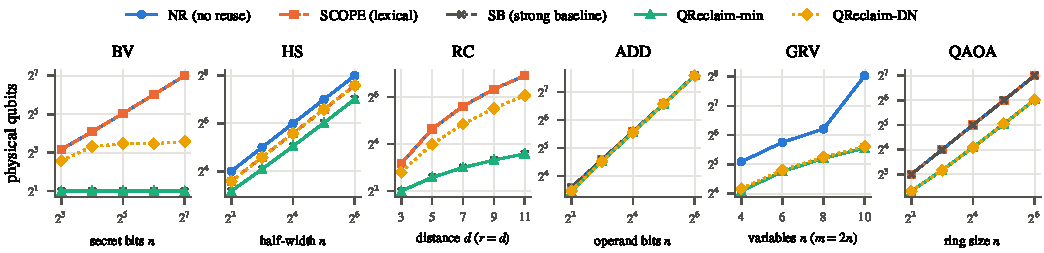
\includegraphics[width=\textwidth]{figures/fig_qubits.pdf}
\caption{Physical qubits (log scale) versus problem size. SB coincides with \QR{}-min except on ADD (DGE) and QAOA (eager placement); SCOPE coincides with NR on BV and RC.}
\label{fig:qubits}
\end{figure*}

\begin{table*}[t]
\caption{Results at the largest size of each family. Width, depth, CX, resets (\QR{}-min/\QR{}-DN) and \QR{} compile time}
\label{tab:main}
\centering
\scriptsize
\setlength{\tabcolsep}{3.2pt}
\begin{tabular}{@{}lrrrrrrrrrrrrr@{}}
\toprule
 & \multicolumn{5}{c}{Width (physical qubits)} & \multicolumn{4}{c}{Depth} & \multicolumn{2}{c}{CX} & Resets & Compile \\
\cmidrule(lr){2-6}\cmidrule(lr){7-10}\cmidrule(lr){11-12}
Benchmark & NR & SCOPE & SB & \QR{}-min & \QR{}-DN & NR & SB & \QR{}-min & \QR{}-DN & NR & \QR{}-min & min/DN & ms \\
\midrule
\inputtable{tables/tab_main.tex}
\bottomrule
\end{tabular}
\end{table*}

\subsection{Width--depth trade-off}
Fig.~\ref{fig:budget} sweeps the budget $B$. Depth falls steeply and reaches the NR depth at \KneeBV\% (BV), \KneeGRV\% (GRV), \KneeRC\% (RC) and \KneeHS\% (HS) of the NR width. \QR{}-DN selects this point automatically and saves \RedDNvsNR\% of the qubits on average with no depth increase on any instance (maximum depth ratio \DNMaxDepth). Under the slow-reset latency model, the duration of \QR{}-DN ranges from \TimeTenMin{} to \TimeTenMax{} times that of NR. Where measured qubits are reused (BV, RC), the remaining resets cost time that unit depth does not show. On such hardware the budget should be chosen with the latency model, which the allocator supports directly.

\begin{figure}[t]
\centering
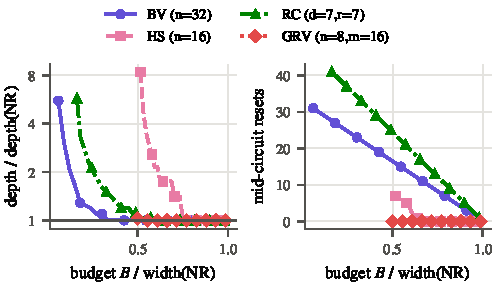
\includegraphics[width=\columnwidth]{figures/fig_budget.pdf}
\caption{Effect of the qubit budget $B$ (normalised by the NR width). Left: depth relative to NR. Right: mid-circuit resets.}
\label{fig:budget}
\end{figure}

\subsection{Leave-one-out ablation}
Table~\ref{tab:ablation} removes one component at a time from the full pipeline. Early measurement is essential for BV and RC (2$\to$33 and 8$\to$49 qubits without it), PALS for BV (2$\to$33), eager placement for QAOA (17$\to$32) and DGE for ADD (47$\to$48). The ERF policy and the two-pass allocation leave width unchanged but reduce depth; GRV, for instance, has depth 1094 with LIFO reuse and 943 without the second pass, against 825 for the full pipeline. On BV, HS, RC and GRV, removing eager placement changes nothing, because PALS hoists lazily placed uncomputations; on HS either one suffices. Eager placement matters exactly when temporaries share inputs, as in QAOA.

\begin{table}[t]
\caption{Leave-one-out ablation: width/depth (BV-32, HS-16, RC-7, ADD-16, GRV-8, QAOA-16)}
\label{tab:ablation}
\centering
\scriptsize
\setlength{\tabcolsep}{2pt}
\begin{tabular}{@{}lrrrrrr@{}}
\toprule
Configuration & BV & HS & RC & ADD & GRV & QAOA \\
\midrule
\inputtable{tables/tab_ablation.tex}
\bottomrule
\end{tabular}
\end{table}

\subsection{External baseline: Qrisp}
Table~\ref{tab:qrisp} compares \QR{}-min with Qrisp on the shared families, with all outputs verified by exact simulation. The comparison is sobering and informative. Qrisp reaches the \emph{same} width on HS and QAOA, which confirms that eager, dependency-aware reclamation is what a mature framework also achieves. It is narrower on GRV and ADD and shallower everywhere. The reason is gate synthesis rather than reclamation: Qrisp implements multi-controlled gates without helper qubits and pairs compute/uncompute Toffolis as cheaper phase-tolerant variants, whereas \QR{} lowers to Barenco V-chains with helpers. Qrisp recycles a measured variable when the programmer deletes it, whereas \QR{} infers measurement-based reuse automatically (BV, RC), checks it statically and exposes it through one budget. Adopting helper-free and phase-tolerant synthesis in \QR{}'s lowering stage is orthogonal to reclamation and is left as future work.

\begin{table}[t]
\caption{\QR{}-min vs.\ Qrisp~0.9.9: width/depth/CX after the same Qiskit lowering}
\label{tab:qrisp}
\centering
\scriptsize
\setlength{\tabcolsep}{3pt}
\begin{tabular}{@{}lrrr@{}}
\toprule
Program & \QR{}-min & Qrisp & Qrisp (workspace 2) \\
\midrule
\inputtable{tables/tab_qrisp.tex}
\bottomrule
\end{tabular}
\end{table}

\subsection{Static checks under bug injection}
Table~\ref{tab:mutation} reports the bug-injection study. All \MutFaulty{} faulty mutants were rejected, so recall is \MutRecall\%, and no accepted mutant failed a run-time $|0\rangle$ assertion. Precision is \MutPrecision\%: \MutFP{} correct mutants were rejected. Each false alarm writes a dependency that later code restores, or that a remaining trace gate never reads, which the first-write deadline $D(a)$ cannot see. Overwriting a control \emph{after} the last use was accepted every time, because eager placement uncomputes before the write. The three diagnostics are:
\begin{lstlisting}[style=ir, breaklines=true]
E1 aliasing violation at [1] `cx x0 -> x0': qubit x0 appears twice in one operation
E2 cannot uncompute ancilla t0: its control x0 is modified by `h x0' at [5] while t0 is still needed at [6]
E3 ancilla t0 can never be reclaimed: `h t0' at [2] puts t0 in superposition, and it is not measured
\end{lstlisting}

\begin{table}[t]
\caption{Bug injection: mutants, faulty (ground truth), TP, FN, FP, TN of the static checks}
\label{tab:mutation}
\centering
\scriptsize
\setlength{\tabcolsep}{3pt}
\begin{tabular}{@{}lrrrrrr@{}}
\toprule
Operator & $n$ & faulty & TP & FN & FP & TN \\
\midrule
\inputtable{tables/tab_mutation.tex}
\bottomrule
\end{tabular}
\end{table}

\subsection{Compilation time and threats to validity}
All main instances compile in at most \MaxCompileMs\,ms, and the linear depth-neutral search takes at most \MaxDNSearchMs\,ms. On inputs scaled to 26{,}594 instructions, a log--log fit of compile time against size has slope \Slope{} (median \UsPerInstr\,$\mu$s per instruction), within 0.5--6.5 times the time of Qiskit's own level-1 transpilation of the output. Threats to validity: depth assumes all-to-all connectivity; SCOPE and SB are our models of prior strategies, not re-implementations of specific tools (Qrisp is the one external tool); the benchmarks are small to medium and chosen to isolate mechanisms; exact simulation is limited to about 20 qubits, beyond which the static validator and the linear and physical checks carry the guarantee.

%% =====================================================================
\section{Conclusion \& Future Work}
\label{sec:concl}
This case study treated qubit reclamation as compiler memory management. A linear IR with static semantics, a basis-state abstract interpretation and an uncomputation-aware liveness analysis decide where reclamation is legal. A unified pass inserts uncomputation, early measurement and resets, and its output is validated statically. An earliest-ready-first linear scan exposes the width--depth trade-off through one budget. \QR{} reduced width by \RedQRvsNR\% on average, and by \RedDNvsNR\% with no depth penalty. It beat a strong baseline built from prior techniques where temporaries share inputs, matched the Qrisp framework's width on two of four shared families, and its static checks found every injected fault. Four extensions are technically meaningful:
\begin{enumerate}
\item \textbf{Recomputation-aware placement.} Chains such as ADD's carries block early reclamation because $\Lst(c_i)\ge P(c_{i+1})$. Adding optional recomputation edges to Eq.~(\ref{eq:lstar}) turns placement into a min-cost reversible pebbling problem under budget $B$~\cite{reqomp}, solvable by ILP for small dependency DAGs and by a fixpoint heuristic otherwise.
\item \textbf{Restoration-aware deadlines.} The false alarms come from writes that later code undoes. Generalising $D(a)$ to a set of open windows, which reopen when the XOR-cancellation test of \S\ref{sec:validate} shows that a dependency has been restored, would accept these programs without losing soundness.
\item \textbf{Reclamation-aware synthesis.} Choosing between helper-based V-chains, helper-free decompositions and phase-tolerant Toffoli pairs inside the hierarchical pass, using the free pool and the budget, would combine Qrisp's synthesis gains with \QR{}'s placement.
\item \textbf{Hardware-aware ERF and feed-forward.} Replace unit latencies with calibrated gate, measurement and reset times and add coupling-map distance to the ERF key. Lift the analyses from one basic block to control-flow graphs with classically controlled branches, which requires a join on the lattice and liveness across branches.
\end{enumerate}

\balance
\bibliographystyle{IEEEtran}
\bibliography{refs}

\end{document}
